\documentclass{standalone}
\usepackage{tikz}
\usepackage{tikz-qtree}
\usepackage[makeroom]{cancel}
\usetikzlibrary{fit}


\begin{document} 
	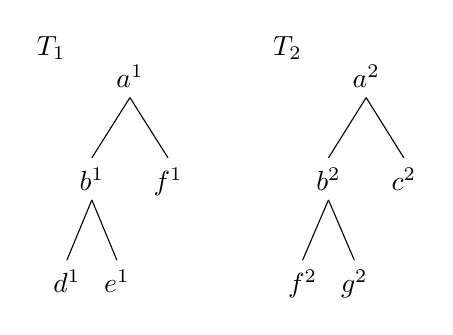
\begin{tikzpicture}[level distance=1.3cm]

	          
		    \node (x) at (-1,0.5) {$T_1$} ;
		    \Tree [.$a^1$
		            [.$b^1$
		                [.$d^1$ ] 
		                [.$e^1$ ] 
		            ] 
		            [.$f^1$ ]
		          ]

	    \begin{scope}[xshift=3cm]
		    \node (x) at (-1,0.5) {$T_2$} ;
		    \Tree [.$a^2$
		            [.$b^2$
		                [.$f^2$ ] 
		                [.$g^2$ ] 
		            ] 
		            [.$c^2$ ]
		          ]
	    \end{scope}

	\end{tikzpicture}
\end{document} 